\section{\sys\ Design}
\label{sec:clio:design}

This section presents the design challenges of building a hardware-based \md\ system and our solutions.

\subsection{Design Challenges and Principles}
Building a hardware-based \md\ platform is a previously unexplored area and introduces new challenges mainly because of restrictions of hardware and the unique requirements of \md.
%Below, we discuss these challenges and our design principles.


\boldpara{Challenge 1: The hardware should avoid maintaining or processing complex data structures}, because unlike software, hardware has limited resources such as on-chip memory and logic cells.
For example, Linux and many other software systems use trees (\eg, the vma tree) for allocation.
Maintaining and searching a big tree data structure in hardware, however, would require huge on-chip memory and many logic cells to perform the look up operation (or alternatively use fewer resources but suffer from performance loss).


\boldpara{Challenge 2: Data buffers and metadata that the hardware uses should be minimal and have bounded sizes}, so that they can be statically planned and fit into the on-chip memory.
Unfortunately, traditional software approaches 
% (usually unawaringly) 
involve various data buffers and metadata that are large and grow with increasing scale.
%; they thus cannot meet our goal.
For example, today's reliable network transports maintain per-connection sequence numbers and buffer unacknowledged packets for packet ordering and retransmission, and they grow with the number of connections.
Although swapping between on-chip and off-chip memory is possible, doing so would increase both tail latency and hardware logic complexity, especially under large scale.
%Thus, it is desirable to resort as little as possible to swapping. 
%Achieving the bounded buffer/state goal is even harder when we simultaneously need to meet our scalability goals.


\boldpara{Challenge 3: The hardware pipeline should be deterministic and smooth},
\ie, it uses a bounded, known number of cycles to process a data unit, and for each cycle, the pipeline can take in one new data unit (from the network).
The former would ensure low tail latency, while the latter would guarantee a throughput that could match network line rate.
Another subtle benefit of a deterministic pipeline is that we can know the maximum time a data unit stays at \MN,
which could help bound the size of certain buffers (\eg, \S\ref{sec:clio:ordering}).
However, many traditional hardware solutions are not designed to be deterministic or smooth, and we cannot directly adapt their approaches.
For example, traditional CPU pipelines could have stalls because of data hazards and have non-deterministic latency to handle memory instructions.

To confront these challenges, we took a clean-slate approach by designing \sys's virtual memory system and network system with the following principles that all aim to eliminate state in hardware or bound their performance and space overhead.

\boldpara{Principle 1: Avoid state whenever possible.}
Not all state in server-based solutions is necessary if we could redesign the hardware.
For example, we get rid of RDMA's MR indirection and its metadata altogether
by directly mapping application process' \rspace\ VAs to PAs (instead of to MRs then to PAs).
%Another type of states that we get rid of is network connections.

\boldpara{Principle 2: Moving non-critical operations and state to software and making the hardware fast path deterministic.}
If an operation is non-critical and it involves complex processing logic and/or metadata, our idea is to move it to the software slow path running in an ARM processor.
For example, VA allocation (\alloc) is expected to be a rare operation
because applications know the disaggregated nature and would typically have only a few large allocations during the execution.
Handling \alloc, however, would involve dealing with complex allocation trees.
We thus handle \alloc\ and \sysfree\ in the software slow path.
Furthermore, in order to make the fast path performance deterministic, we {\em decouple} all slow-path tasks from the performance-critical path by {\em asynchronously} performing them in the background.
%Note that page fault is a relatively critical operation, as all first accesses to allocated virtual pages will cause a fault, and applications like serverless computing could access large amounts of (new) memory in a short period of time.



\boldpara{Principle 3: Shifting functionalities and state to \CN{}s.}
While hardware resources are scarce at \MN{}s, \CN{}s have sufficient memory and processing power, and it is faster to develop functionalities in \CN\ software.
A viable solution is to shift state and functionalities from \MN{}s to \CN{}s.
The key question here is how much and what to shift.
%; shifting too much would make \sys\ similar to \pdm\ and suffer from various performance and security issues of \pdm.
Our strategy is to shift functionalities to \CN{}s only if doing so 1) could largely reduce hardware resource consumption at \MN{}s, 2) does not slow down common-case foreground data operations, 3) does not sacrifice security guarantees, and 4) adds bounded memory space and CPU cycle overheads to \CN{}s.
As a tradeoff, the shift may result in certain uncommon operations (\eg, handling a failed request) being slower.
%Our insight here is that we can if a shift results in performance tradeoff only for uncommon cases
%For example, traditional reliable network stacks require maintaining 

\boldpara{Principle 4: Making off-chip data structures efficient and scalable.}
Principles 1 to 3 allow us to reduce \MN\ hardware to only the most essential functionalities and state. 
We store the remaining state in off-chip memory and cache a fixed amount of them in on-chip memory.
Different from most caching solutions, our focus is to make the access to off-chip data structure fast and scalable,
\ie, all cache misses have bounded latency regardless of the number of client processes accessing an \MN\ or the amount of physical memory the \MN\ hosts.

\boldpara{Principle 5: Making the hardware fast path smooth by treating each data unit independently at \MN.}
If data units have dependencies (\eg, must be executed in a certain order), then the fast path cannot always execute a data unit when receiving it.
To handle one data unit per cycle and reach network line rate, we make each data unit independent by including all the information needed to process a unit in it and by allowing \MN{}s to execute data units in any order that they arrive.
%there is no dependency check across data units at \MN{}s.
To deliver our consistency guarantees, we opt for enforcing request ordering at \CN{}s before sending them out.

The rest of this section presents how we follow these principles to design \sys's three main functionalities: memory address translation and protection, page fault handling, and networking. We also briefly discuss our offloading support.

\subsection{Scalable, Fast Address Translation}
\label{sec:clio:addr-trans}
%Similar to traditional virtual memory addressing, we use fix-size pages as VA/PA allocation and address translation unit, while data accesses are in the unit of byte.
Similar to traditional virtual memory systems, we use fix-size pages as address allocation and translation unit, while data accesses are in the granularity of byte.
Despite the similarity in the goal of address translation,
%(\ie, translating a virtual page to a physical page number),
the radix-tree-style, per-address space page table design used by all current architectures~\cite{ecuckoo-asplos20} does not fit \md\ for two reasons.
First, each request from the network could be from a different client process. If each process has its own page table, \MN\ would need to cache and look up many page table roots, causing additional overhead.
Second, a multi-level page table design requires multiple DRAM accesses when there is a translation lookaside buffer (TLB) miss~\cite{hashpgtable-sigmetrics16}.
TLB misses will be much more common in a \md\ environment, since with more applications sharing an \MN, the total working set size is much bigger than that in a single-server setting, while the TLB size in an \MN\ will be similar or even smaller than a single server's TLB (for cost concerns). To make matters worse, each DRAM access is more costly for systems like RDMA NIC which has to cross the PCIe bus to access the page table in main memory~\cite{Pythia,pcie-sigcomm}.

\ulinebfpara{Flat, single page table design (Principle 4).}~~
We propose a new {\em overflow-free} hash-based page table design that sets the total page table size according to the physical memory size 
and bounds \textit{address translation to at most one DRAM access}.
Specifically, we store {\em all} page table entries (PTEs) from {\em all} processes in a single hash table 
whose size is proportional to the physical memory size of an \MN. 
The location of this page table is fixed in the off-chip DRAM and is known by the fast path address translation unit, thus avoiding any lookups.
%We create the page table to always have enough entries to cover the entire physical memory.
As we anticipate applications to allocate big chunks of VAs in their \rspace, we use huge pages and support a configurable set of page sizes.
%Each PTE is 8 bytes, 
With the default 4\MB\ page size, the hash table consumes only 0.4\%\ of the physical memory.
%For example, for 1\TB\ physical memory and 4\MB\ page size, the whole page table is only 4\MB\ (each PTE is 8 bytes).

{
\begin{figure}[t]
\begin{center}
\centerline{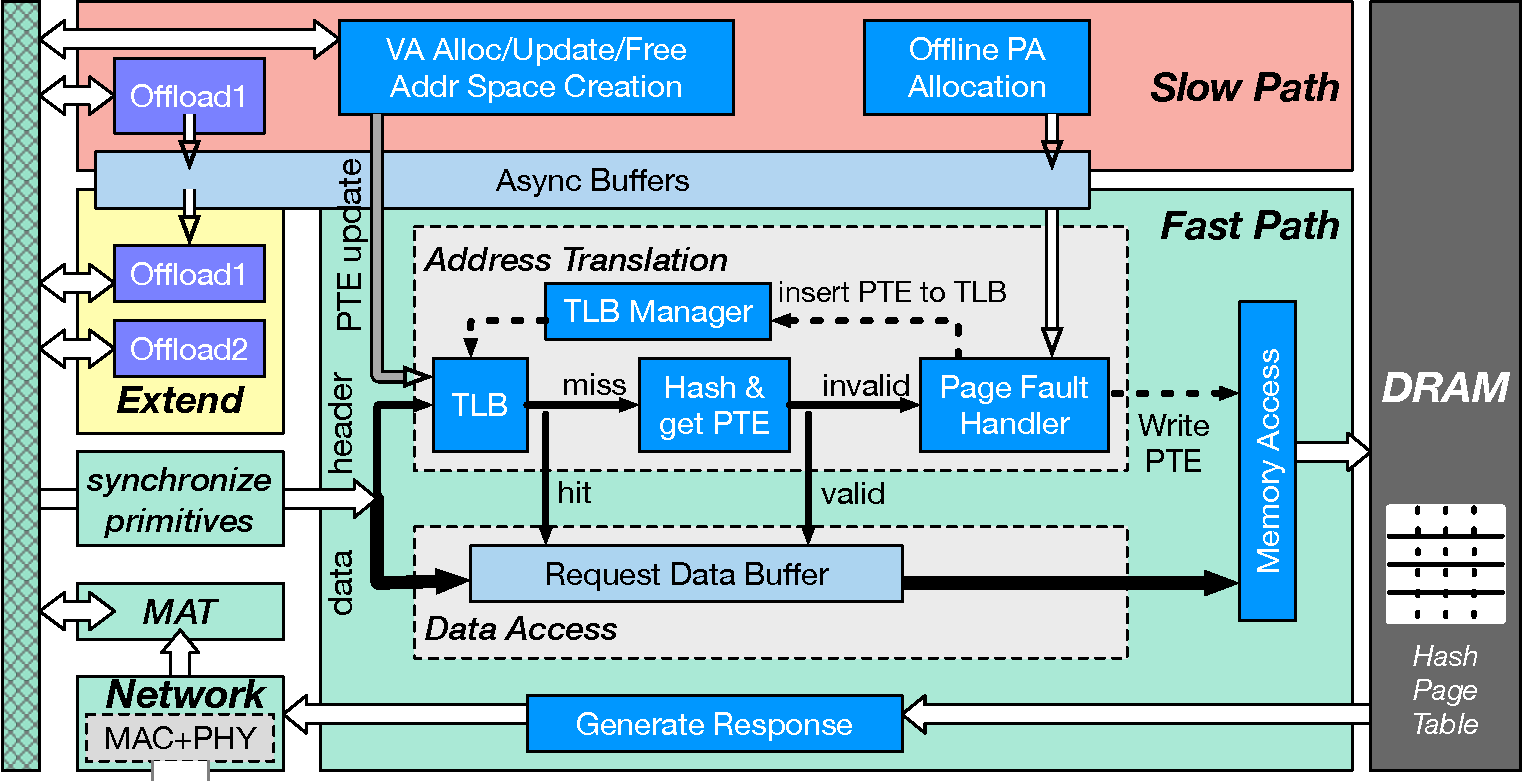
\includegraphics[width=\columnwidth]{Figures/CoreMem.pdf}}
%\vspace{-0.1in}
\mycaption{fig-coremem}{\sysboard\ Design.}
{
%Thick lines represent data payload. Thin lines represent header information.
%Double line represents metadata from ARM.
%Dashed line represents internal operations.
Green, yellow, and red areas are anticipated to be built with 
ASIC, FPGA, and low-power cores.
}
\end{center}
%\end{minipage}
%\vspace{-0.2in}
\end{figure}
}


The hash value of a VA and its PID is used as the index to determine which hash bucket the corresponding PTE goes to.
Each hash bucket has a fixed number of ($K$) slots.
To access the page table, we always fetch
the entire bucket including all $K$ slots in a single DRAM access.
%Normally, a hash table with fixed slots will have an overflow problem because of hash conflicts (\eg, when more than $K$ VA+PID combinations have the same hash value).

A well-known problem with hash-based page table design is hash collisions that could overflow a bucket.
Existing hash-based page table designs rely on collision chaining~\cite{TransCache-isca10} or open addressing~\cite{hashpgtable-sigmetrics16} to handle overflows, both require multiple DRAM accesses or even costly software intervention.
In order to bound address translation to at most one DRAM access, we use a novel technique to avoid hash overflows at \textit{VA allocation time}.

\ulinebfpara{VA allocation (Principle 2).}~~
The slow path software handles \alloc\ requests and allocates VA.
The software allocator maintains a per-process VA allocation tree that records allocated VA ranges and permissions, similar to the Linux vma tree~\cite{linux-rb-vma}.
To allocate size $k$ of VAs, it first finds an available address range of size $k$ in the tree.
It then calculates the hash values of the virtual pages in this address range
and checks if inserting them to the page table would cause any hash overflow. 
If so, it %marks the failed virtual pages in the tree as ``unusable'' and 
does another search for available VAs.
These steps repeat until it finds a valid VA range that does not cause hash overflow.
%It then send these VA page numbers (VPN) to the hardware fast path, which inserts the corresponding PTEs (invalid PTEs without PAs) to the page table. The last step is crucial for fast page fault handling in the hardware.
%It then send these VA page numbers and their permissions to the hardware fast path, which establishes the corresponding PTEs (with invalid state, \ie, with permission set up but no PAs). %The last step is crucial for fast page fault handling in the hardware as it enables in-line VA permission checking.

Our design trades potential retry overhead at allocation time (at the slow path) for better run-time performance and simpler hardware design (at the fast path).
% core-memory implementation.
This overhead is manageable because
1) each retry takes only a few microseconds with our implementation (\S\ref{sec:clio:impl}),
%is fast even when running at ARM processor (\mus\ level), 
2) we employ huge pages, which means fewer pages need to be allocated, 
3) we choose a hash function that has very low collision rate~\cite{lookup3-wiki},
and 4) we set the page table to have extra slots (2\x\ by default) which absorbs most overflows.
%and 5) the \sys\ 64-bit virtual address space is huge.
%In fact, none of our evaluated application's \alloc\ requests ever require retry, even when the \alloc\ size is as huge as 1\TB.
We find no conflicts when memory is below half utilized and has only up to 60 retries when memory is close to full (Figure~\ref{fig-alloc-conflict}).

\ulinebfpara{TLB.}~~
%and its consistency with the page table.}
\sys\ implements a TLB in a fix-sized on-chip memory area and looks it up using content-addressable-memory in the fast path.
%and use LRU for replacement, 
On a TLB miss, the fast path fetches the PTE from off-chip memory and inserts it to the TLB by replacing an existing TLB entry with the LRU policy.
When updating a PTE, the fast path also updates the TLB, in a way that ensures the consistency of inflight operations.
%
%As with traditional TLB, \sys\ also faces a consistency problem between TLB and the page table.
%Traditionally, the OS needs to shootdown TLBs after modifying PTEs~\cite{tlbshootdown-eurosys20}.
%\sys's software slow path is the party that modifies a PTE, \eg, deleting a PTE when handling \sysfree.
%With our separate fast- and slow-path design, there could be potential %consistency problems when both paths try to access/modify the page table.
%The first consistency problem happens when the slow path needs to update the %page table (\eg, when handling a \sysfree).
%between slow-path generated PTE changes (update or delete) and fast-path TLB.
%Instead of letting the slow path change the page table in DRAM and shootdown the TLB in the on-chip memory,
%we let the hardware fast path pipeline handle all page table {\em and} TLB modifications.
%With the latter, it is easier to ensure the consistency of inflight fast-path operations, as they are in the same pipeline as the TLB/page-table modification logic.
%\zhiyuan{Is the above correct?}
%If it directly applies the change to the page table in DRAM, then the TLB will be inconsistent.
%Today's computer relies on the OS to perform costly~\cite{XXX} TLB shootdowns for TLB consistency.
%Following our design of only having the fast path managing TLB,
%To solve this problem, we adopt a simple principle: the fast path is the only unit accessing and changing TLB {\em and} the page table.
%We use a different approach where
%Thus, the slow path hands over its PTE change requests to the fast path, 
%which performs both the TLB change and the PTE change in its pipeline in a way that is consistent for inflight fast-path operations.

\ulinebfpara{Limitation.}~~
A downside of our overflow-free VA allocation design is that it cannot guarantee that a specific VA can be inserted into the page table. This is not a problem for regular VA allocation but could be problematic for allocations that require a fixed VA (\eg, \texttt{mmap(MAP\_FIXED})). 
Currently, \sys\ finds a new VA range if the user-specified range cannot be inserted into the page table. Applications that must map at fixed VAs (\eg, libraries) will need to use \CN-local memory.


\subsection{Low-Tail-Latency Page Fault Handling}

A key reason to disaggregate memory is to consolidate memory usages on less DRAM so that memory utilization is higher and the total monetary cost is lower (\textbf{R1}). Thus, remote memory space is desired to run close to full capacity, and we allow memory over-commitment at an \MN, necessitating page fault handling. Meanwhile, applications like JVM-based ones allocate a large heap memory space at the startup time and then slowly use it to allocate smaller objects. Similarly, many existing far-memory systems~\cite{Tsai20-ATC,AIFM,FaRM} allocate a big chunk of remote memory and then use different parts of it for smaller objects to avoid frequently triggering the slow remote allocation operation.
In these cases, it is desirable for a \md\ system to delay the allocation of physical memory to when the memory is actually used (\ie, {\em on-demand} allocation) or to ``reshape'' memory~\cite{cliquemap-sigcomm21} during runtime, necessitating page fault handling.

Page faults are traditionally signaled by the hardware and handled by the OS. %, and they can happen when a PTE is invalid (VA created, PA not allocated)
%or when there is a permission violation. 
%A common case of page faults are {\em first-time accesses}, which requires on-demand physical memory allocation.
%While the latter is uncommon, the former happens at every initial access to a VA and could be common 
%First-time accesses can be common in applications like serverless computing and microservices which frequently start many short running processes and incur many initial-access page faults.
%Unfortunately, today's page fault handling mechanism is slow because of the costly interrupt and trap-to-kernel process.
This is a slow process because of the costly interrupt and kernel-trapping flow.
For example, a remote page fault via RDMA costs 16.8\ms\ from our experiments using Mellanox ConnectX-4.
To avoid page faults, most RDMA-based systems pre-allocate big chunks of physical memory and pin them physically.
However, doing so results in memory wastes and makes it hard for an \MN\ to pack more applications, violating \textbf{R1} and \textbf{R2}.

%\boldpara{Decoupling PA allocation from page fault handling.}
%To meet \textbf{R2}, \textbf{R3}, and \textbf{R6}, 
We propose to {\em handle page faults in hardware and with bounded latency}\textemdash a {\em constant three cycles} to be more specific with our implementation of \sysboard.
%Achieving this performance is not easy.
%While handling permission-violation faults in hardware is easy (just by sending an error message as the request response),
%Particularly, 
Handling initial-access faults in hardware is challenging, as initial accesses require PA allocation, which is a slow operation that involves manipulating complex data structures.
Thus, we handle PA allocation in the slow path (\textbf{Challenge 1}).
However, if the fast-path page fault handler has to wait for the slow path to generate a PA for each page fault,
it will slow down the data plane.
%As allocation is performed by ARM, fetching the allocation results via the slow path between FPGA and ARM would hugely affect foreground performance.

To solve this problem, we propose an asynchronous design to shift PA allocation off the performance-critical path (\textbf{Principle 2}).
Specifically, we maintain a set of {\em free physical page numbers} in an {\em async buffer},
which the ARM continuously fulfills by finding free physical page addresses and reserving them without actually using the pages. % actual allocation.
During a page fault, the page fault handler simply fetches a pre-allocated physical page address. % of the corresponding page size.
%This asynchronous design enables us to avoid the long wait for ARM to do an allocation on the fly.
Note that even though a single PA allocation operation has a non-trivial delay, 
the throughput of generating PAs and filling the async buffer is higher than network line rate.
%the throughput of generating PAs and filling the async buffer is higher than page fault rate.
Thus, the fast path can always find free PAs in the async buffer in time.
After getting a PA from the async buffer and establishing a valid PTE, %(promoted from the specially marked invalid state), 
the page fault handler performs three tasks in parallel: 
writing the PTE to the off-chip page table, inserting the PTE to the TLB,
and continuing the original faulting request.
This parallel design hides the performance overhead of the first two tasks, allowing foreground requests to proceed immediately.

A recent work~\cite{lee-isca20} also handles page faults in hardware. 
%Its goal, however, is to accelerate data fetching from storage and focuses 
Its focus is on the complex interaction with kernel and storage devices, and it is a simulation-only work. \sys\ uses a different design for handling page faults in hardware with the goal of low tail latency, and we built it in FPGA.

\ulinebfpara{Putting the virtual memory system together.}~~
We illustrate how \sysboard{}'s virtual memory system works using a simple example of allocating some memory and writing to it.
The first step (\alloc) is handled by the slow path, which allocates a VA range by finding an available set of slots in the hash page table.
The slow path forwards the new PTEs to the fast path, which inserts them to the page table.
At this point, the PTEs are invalid.
This VA range is returned to the client.
When the client performs the first write, the request goes to the fast path.
There will be a TLB miss, followed by a fetch of the PTE.
Since the PTE is invalid, the page fault handler will be triggered,
which fetches a free PA from the async buffer and establishes the valid PTE.
It will then execute the write, update the page table, and insert the PTE to TLB.

\subsection{Asymmetric Network Tailored for \md}
\label{sec:clio:network}
With large amounts of research and development efforts, today's data-center network systems are highly optimized in their performance.
Our goal of \sys's network system is unique and fits \md's requirements\textemdash minimizing the network stack's hardware resource consumption at \MN{}s and achieving great scalability while maintaining similar performance as today's fast network.
Traditional software-based reliable transports like Linux TCP incurs high performance overhead.
Today's hardware-based reliable transports like RDMA are fast, but they require a fair amount of on-chip memory to maintain state, \eg, per-connection sequence numbers, congestion state~\cite{TONIC}, and bitmaps~\cite{IRN,MELO-APNet}, not meeting our low-cost goal.
%and buffers (\eg, the unacknowledged packet buffer, packet reorder buffer)
%Maintaining them in on-chip memory is not a viable solution because of \textbf{Challenge 2} (cost). 

Our insight is that different from general-purpose network communication where each endpoint can be both the sender (requester) and the receiver (responder) that exchange general-purpose messages,
\MN{}s only respond to requests sent by \CN{}s (except for memory migration from one \MN\ to another \MN\ (\S\ref{sec:clio:dist}), in which case we use another simple protocol to achieve the similar goal).
Moreover, these requests are all memory-related operations that have their specific properties.
With these insights, we design a new network system with two main ideas.
%and does so without the need to change any existing data-center network infrastructure.
Our first idea is to maintain transport logic, state, and data buffers only at \CN{}s,
essentially making \MN{}s ``transportless'' (\textbf{Principle 3}). 
%\footnote{1RMA~\cite{1RMA}, a recent server-based remote memory system, onloads most of its retransmission and congestion logic from the NIC to the host CPU. As a result, 1RMA's NIC is simple.
%and connectionless. 
%However, 1RMA relies on a companion host to function, violating the ``server-less'' goal of \MN{}s.}.
Our second idea is to relax the reliability of the transport and instead enforce ordering and loss recovery at the memory request level, so that \MN{}s' hardware pipeline can process data units as soon as they arrive (\textbf{Principle 5}).

With these ideas, we implemented a transport in \syslib\ at \CN{}s. \syslib\ bypasses the kernel to directly issue raw Ethernet requests to an Ethernet NIC.
\CN{}s use regular, commodity Ethernet NICs and regular Ethernet switches to connect to \MN{}s.
\MN{}s include only standard Ethernet physical, link, and network layers and a slim layer for handling corner-case requests (\S\ref{sec:clio:ordering}).
%\yizhou{We use lossless Ethernet enabled by Priority Flow Control (PFC) as it reduces packet loss and retry rate. PFC comes with a set of issues~\cite{DCQCN-sigcomm15,hpcc-sigcomm19}. Hence we design our protocol to avoid triggering it as much as possible.}
We now describe our detailed design.

%Both \CN{}s and \MN{}s only need standard Ethernet physical and link layers in the hardware.
%Thus, \CN{} servers can continue using regular Ethernet-based NICs, and \MN{}s can be built with low cost.

\ulinebfpara{Removing connections with request-response semantics.}
Connections (\ie, QPs) are a major scalability issue with RDMA.
Similar to recent works~\cite{Homa,1RMA}, we make our network system connection-less using request-response pairs.
Applications running at \CN{}s directly initiate \sys\ APIs to an \MN\ without any connections.
%Since all \sys\ operations are in the RPC style initiated by client servers, \ie, sending read/write requests and getting data/response back,
%Similar to Homa~\cite{Homa}, 
\syslib\ assigns a unique request ID to each request. The \MN\ attaches the same request ID when sending the response back. \syslib\ uses responses as ACKs and matches a response with an outstanding request using the request ID.
Neither \CN{}s nor \MN{}s send ACKs.
%the response of each \sys\ request as the ACK and matches it to the request using a request ID.

\ulinebfpara{Lifting reliability to the memory request level.}
Instead of triggering a retransmission protocol for every lost/corrupted packet at the transport layer, 
\syslib\ retries the entire memory request if any packet is lost or corrupted in the sending or the receiving direction.
On the receiving path, \MN{}'s network stack only checks a packet's integrity at the link layer. If a packet is corrupted, the \MN\ immediately sends a NACK to the sender \CN.
%, otherwise the packet is delivered to the address translation module.
\syslib\ retries a memory request if one of three situations happens: a NACK is received, the response from \MN\ is corrupted, or no response is received within a \texttt{TIMEOUT} period.
%dynamic retransmission timeout (RTO) period. The RTO is computed %on a per-path basis 
%using the moving average of prior end-to-end RTTs.
%We also avoid complex logic/states to detect lost packets and simply determine the failure of a request if no response is received in a \texttt{TIMEOUT} period.
%We rely on standard link-layer mechanisms to correct packet corruptions and report uncorrectable ones~\cite{FEC}.
In addition to lifting retransmission from transport to the request level, we also lift ordering to the memory request level
and allow out-of-order packet delivery (see details in \S\ref{sec:clio:ordering}).

%\boldpara{\CN-controlled congestion and incast.}
\ulinebfpara{\CN-managed congestion and incast control.}
Our goal of controlling congestion in the network and handling incast that can happen both at a \CN\ and an \MN\ is to minimize state at \MN.
To this end, we build the entire congestion and incast control at the \CN\ in the \syslib.
%\sys\ performs congestion control (CC) at \syslib\ to 1) keep \MN{}s stateless, and 2) make it easy for users to change the CC policy.
%Our current CC policy exploits the fact that \CN{}s know the sizes of both requests and expected responses to control congestion on both the outgoing and incoming directions at \CN{}s.
To control congestion, \syslib\ adopts a simple delay-based, reactive policy that uses end-to-end RTT delay as the congestion signal, similar to recent sender-managed, delay-based mechanisms~\cite{mittal2015timely,swift-sigcomm,1RMA}.
%We onload CC and implement it using software to keep it flexible and easier to adopt new policies. To this end, we use a simple delay-based, reactive CC mechanism at \syslib.
%End-to-end RTT delay is our primary congestion signal.
%Delay has been shown to be an effective and robust signal in the heterogeneous datacenter environments~\cite{mittal2015timely,swift-sigcomm,1RMA}.
%It requires no special switch features such as ECN~\cite{DCQCN} or INT~\cite{HPCC}.
Each \CN\ maintains one congestion window, \textit{cwnd}, per \MN\ 
%which is shared by all processes accessing the \MN.
%It 
that controls the maximum number of outstanding requests that can be made to the \MN\ from this \CN.
We adjust \textit{cwnd} based on measured delay using a standard Additive Increase Multiplicative Decrease (AIMD) algorithm.

To handle incast to a \CN, we exploit the fact that the \CN{} knows the sizes of expected responses for the requests that it sends out and that responses are the major incoming traffic to it.
Each \syslib\ maintains one incast window, \textit{iwnd}, which controls the maximum bytes of expected responses. \syslib\ sends a request only when both \textit{cwnd} and \textit{iwnd} have room.

Handling incast to an \MN\ is more challenging, as we cannot throttle incoming traffic at the \MN\ side or would otherwise maintain state at \MN{}s.
To have \CN{}s handle incast to \MN{}s, we draw inspiration from Swift~\cite{swift-sigcomm} by allowing \textit{cwnd} to fall below one packet when long delay is observed at a \CN. For example, a \textit{cwnd} of 0.1 means that the \CN\ can only send a packet within 10 RTTs.
Essentially, this situation happens when the network between a \CN\ and an \MN\ is really congested, and the only way is to slow the sending speed.

\subsection{Request Ordering and Data Consistency}
\label{sec:clio:ordering}

As explained in \S\ref{sec:clio:abstraction}, \sys\ supports both synchronous and asynchronous remote memory APIs, with the former following a sequential, one-at-a-time order in a thread and the latter following a release order in a thread.
Furthermore, \sys\ provides synchronization primitives for inter-thread consistency.
We now discuss how \sys\ achieves these correctness guarantees by presenting our mechanisms for handling intra-request intra-thread ordering, inter-request intra-thread ordering, inter-thread consistency, and retries.
At the end, we will provide the rationales behind our design.

One difficulty in designing the request ordering and consistency mechanisms is our relaxed network ordering guarantees, 
which we adopt to minimize the hardware resource consumption for the network layer at \MN{}s (\S\ref{sec:clio:network}).
On an asynchronous network, it is generally hard to guarantee any type of request ordering when there can be multiple outstanding requests (either multiple threads accessing shared memory or a single thread issuing multiple asynchronous APIs). It is even harder for \sys\ because we aim to make \MN\ stateless as much as possible.
%Allowing memory requests to be asynchronous Ensuring even a weaker consistency level like release consistency is hard when the network can reorder and drop packets and when we aim to minimize states at \MN{}s.
Our general approaches are 1) using \CN{}s to ensure that no two concurrently outstanding requests are dependent on each other, and 2) using \MN{}s to ensure that every user request is only executed once even in the event of retries.

%\zhiyuan{We design our consistency model based on the requirements of disaggregation and the efficiency of hardware design.
%Most desegregation use cases (e.g. with local caches) rarely send out memory access requests with dependency, so strict ordering can be an overkill; This allows us to apply released consistency model and simplify hardware design} 

%\zhiyuan{We apply an released consistency similar to ARMv8, which allows 
%which dependent requests in Clio only includes memory fences and requests that operates on the same address. We also provide synchronization primitives, \syslock and \fence between threads. The execution order of other requests and request from different threads. can be reordered at \CN{}, network or \MN{}.}

%\zhiyuan{We apply two rules to implement our consistency model. First, for a client, all committed but not completed requests must not have dependency; Second, At MN side, all request must be executed and only executed once. The rules ensures the correctness of the implementation.}

\ulinebfpara{Allowing intra-request packet re-ordering (T1).}
%\zhiyuan{We use client side libraries to ensure first rule.}
%Packet reordering can happen in the network, \eg, due to data-center multipath routing~\cite{ECMP}. %which can happen at the link layer.
A request or a response in \sys\ can contain multiple link-layer packets. 
Enforcing packet ordering above the link layer normally requires maintaining state (\eg, packet sequence ID) at both the sender and the receiver.
To avoid maintaining such state at \MN{}s,
our approach is to deal with packet reordering only at \CN{}s in \syslib\ (\textbf{Principle 3}).
Specifically, \syslib\ splits a request that is bigger than link-layer maximum transmission unit (MTU) into several link-layer packets
and attaches a \sys\ header to each packet, which includes sender-receiver addresses, a request ID, and request type.
This enables the \MN{} to treat each packet independently (\textbf{Principle 5}).
It executes packets as soon as they arrive, even if they are not in the sending order.
This out-of-order data placement semantic is in line with RDMA specification~\cite{IRN}. 
Note that only write requests will be bigger than MTU, and the order of data writing within a write request does not affect correctness as long as proper {\em inter-request} ordering is followed.
When a \CN\ receives multiple link-layer packets belonging to the same request response, 
\syslib\ reassembles them before delivering them to the application.


\ulinebfpara{Enforcing intra-thread inter-request ordering at \CN\ (T2).}
Since only one synchronous request can be outstanding in a thread, there cannot be any inter-request reordering problem.
%Synchronous requests follow strict program order with only at most one outstanding request.
%and we do not need to take any special measurement for synchronous request ordering.
On the other hand, there can be multiple outstanding asynchronous requests.
Our provided consistency level disallows concurrent asynchronous requests that are dependent on each other (WAW, RAW, or WAR).
In addition, all requests must complete before \release.



We enforce these ordering requirements at \CN{}s in \syslib\ instead of at \MN{}s (\textbf{Principle 3}) for two reasons.
First, enforcing ordering at \MN{}s requires more on-chip memory and complex logic in hardware.
Second, even if we enforce ordering at \MN{}s, network reordering would still break end-to-end ordering guarantees.
%To enforce ordering for asynchronous operations at the client side, 

Specifically, \syslib\ keeps track of all inflight requests and matches every new request's virtual page number (VPN) to the inflight ones'. 
If a WAR, RAW, or WAW dependency is detected, \syslib\ blocks the new request until the conflicting request finishes.
When \syslib\ sees a \release\ operation, it waits until all inflight requests return or time out.
We currently track dependencies at the page granularity mainly to reduce tracking complexity and metadata overhead. The downside is that false dependencies could happen (\eg, two accesses to the same page but different addresses).
False dependencies could be reduced by dynamically adapting the tracking granularity if application access patterns are tracked\textemdash we leave this improvement for future work.
%tailored for application needs.
%In reality, this is not a problem, as with a low-latency system like \sys, the amount of outstanding requests is small and the chance of two outstanding requests accessing the same page is extremely rare.
%, which largely depends on application usage.
%Intuitively, it is problematic for data structure systems~\cite{AIFM} with small granularity access, but works well for others with larger accesses. We leave this optimization for future work.
%For synchronous operations, \syslib\ only returns when a request gets a response, effectively achieving strict ordering.

\ulinebfpara{Inter-thread/process consistency (T3).}
%\zhiyuan{At the \MN{} side, we ensures the semantic of execute once.}
%\zhiyuan{Move the retry to earlier position?}
Multi-threaded or multi-process concurrent programming on \sys\ could use the synchronization primitives \sys\ provides to ensure data consistency (\S\ref{sec:clio:abstraction}).
%, \eg, by protecting a critical section using \syslock.
We implemented all synchronization primitives like \syslock\ and \fence\ at \MN,
because they need to work across threads and processes that possibly reside on different \CN{}s.
Before a request enters either the fast or the slow paths, 
\MN\ checks if it is a synchronization primitive.
%an atomic operation or a \fence.
For primitives like \syslock\ that internally is implemented using atomic operations like \texttt{TAS}, \MN\ blocks future atomic operations until the current one completes.
For \fence, \MN\ blocks all future requests until all inflight ones complete.
Synchronization primitives are one of the only two cases where \MN\ needs to maintain state.
%As these operations operation executes in bounded time, the hardware resources for states are bounded.
As these operations are infrequent and each of these operations executes in bounded time, the hardware resources for maintaining their state are minimal and bounded.

\ulinebfpara{Handling retries (T4).}
\syslib\ retries a request after a \texttt{TIMEOUT} period without receiving any response. Potential consistency problems could happen as \sysboard\ could execute a retried write after the data is written by another write request thus undoing this other request's write. Such situations could happen when the original request's response is lost or delayed and/or when the network reorders packets. 
%Such situation would violate \sys's consistency guarantees.
%Such situations could happen because the network could reorder packets and because we support multiple concurrent processes sharing the same data.
%
We use two techniques to solve this problem.

First, \syslib\ attaches a new request ID to each retry, essentially making it a new request with its own matching response. Together with \syslib's ordering enforcement, it ensures that there is only one outstanding request (or a retry) at any time.
Second, we maintain a small buffer at \MN\ to record the request IDs of recently executed writes and atomic APIs and the results of the atomic APIs. A retry attaches its own request ID and the ID of the failed request. If \MN\ finds a match of the latter in the buffer, it will not execute the request. For atomic APIs, it sends the cached result as the response. We set this buffer's size to be 3$\times$\texttt{TIMEOUT}$\times$\textit{bandwidth}, which is 30\KB\ in our setting. It is one of the only two types of state \MN\ maintains and does not affect the scalability of \MN, since its size is statically associated with the link bandwidth and the \texttt{TIMEOUT} value.
With this size, the \MN\ can ``remember'' an operation long enough for two retries from the \CN. Only when both retries and the original request all fail, the \MN\ will fail to properly handle a future retry. This case is extremely rare~\cite{Homa}, and we report the error to the application, similar to \cite{Kalia14-RDMAKV,1RMA}.

\ulinebfpara{Why T1 to T4?}
We now briefly discuss the rationale behind why we need all T1 to T4 to properly deliver our consistency guarantees. 
First, assume that there is no packet loss or corruption (\ie, no retry) but the network can reorder packets. 
In this case, using T1 and T2 alone is enough to guarantee the proper ordering of \sys\ memory operations, since they guarantee that network reordering will only affect either packets within the same request or requests that are not dependent on each other.
T3 guarantees the correctness of synchronization primitives since the \MN\ is the serialization point and is where these primitives are executed.
Now, consider the case where there are retries.
Because of the asynchronous network, a timed-out request could just be slow and still reach the \MN, either before or after the execution of the retried request. If another request is executed in between the original and the retried requests, inconsistency could happen (\eg, losing the data of this other request if it is a write). The root cause of this problem is that one request can be executed twice when it is retried.
T4 solves this problem by ensuring that the \MN\ only executes a request once even if it is retried.


\subsection{Extension and Offloading Support}
\label{sec:clio:extended}
To avoid network round trips when working with complex data structures and/or performing data-intensive operations,
we extend the core \MN\ to support application computation offloading in the extend path.
%which includes an FPGA chip and the ARM processor.
%We only have space to give a high-level overview of the extend path, leaving details to a follow-on paper.
Users can write and deploy application offloads both in FPGA and in software (run in the ARM).
%An offload can either be the handler of a high-level API (\eg, pointer chasing) or an entire function (\eg, data filtering).
To ease the development of offloads, \sys\ offers the same virtual memory interface as the one to applications running at \CN{}s.
Each offload has its own PID and virtual memory address space, and they use the same virtual memory APIs (\S\ref{sec:clio:abstraction}) to access on-board memory. It could also share data with processes running at \CN{}s in the same way that two \CN\ processes share memory.
%Developing offloads is thus closer to traditional multi-threaded programming (in terms of memory accesses).
Finally, an offload’s data and control paths could be split to FPGA and ARM and use the same async-buffer mechanism for communication between them. 
These unique designs made developing computation offloads easier and closer to traditional multi-threaded software programming.


\subsection{Distributed \MN{}s}
\label{sec:clio:dist}
Our discussion so far focused on a single \MN\ (\sysboard).
To more efficiently use remote memory space and to allow one application to use more memory than what one \sysboard\ can offer, we extend the single-\MN\ design to a distributed one with multiple \MN{}s.
Specifically, an application process' \rspace\ can span multiple \MN{}s, and one \MN\ can host multiple \rspace{}s.
We adopt LegoOS' two-level distributed virtual memory management approach to manage distributed \MN{}s in \sys.
A global controller manages \rspace{}s in coarse granularity (assigning 1\GB\ virtual memory regions to different \MN{}s).
Each \MN\ then manages the assigned regions at fine granularity.

The main difference between LegoOS and \sys's distributed memory system is that in \sys, each \MN\ can be over-committed (\ie, allocating more virtual memory than its physical memory size), and when an \MN\ is under memory pressure, it migrates data to another \MN\ that is less pressured (coordinated by the global controller).
The traditional way of providing memory over-commitment is through memory swapping, which could be potentially implemented by swapping memory between \MN{}s. 
However, swapping would cause performance impact on the data path and add complexity to the hardware implementation.
Instead of swapping, we \textit{proactively} migrate a rarely accessed memory region to another \MN\ when an \MN\ is under memory pressure (its free physical memory space is below a threshold).
During migration, we pause all client requests to the region being migrated.
With our 10\Gbps\ experimental board, migrating a 1\GB\ region takes 1.3 second.
Migration happens rarely and, unlike swapping, happens in the background.
Thus, it has little disturbance to foreground application performance.


